\documentclass{article}
\usepackage[utf8]{inputenc}

\title{%
  Sistema de Avaliação de Discente\\
  \large utilizando lógica\\
    Fuzzy}

\author{Daniel Ferreira, Ivan Carlos, Rodrigo de Paula}
\date{October 2021}

\usepackage{natbib}
\usepackage{amsmath}  % matemática

\usepackage{blindtext} % links
\usepackage{hyperref}  % links

\usepackage{graphicx}
\usepackage{geometry}
\usepackage[utf8]{inputenc}
\usepackage[T1]{fontenc}
\usepackage[brazil]{babel}

%\geometry{left=2.5cm,right=2.5cm,top=2.5cm,bottom=2.5cm}

\begin{document}

\maketitle

\section{Descrição do trabalho}

O trabalho consiste em projetar, implementar e mostrar
funcionando um sistema de avaliação que utilize lógica difusa
(fuzzy), para gerar a média final dos alunos de uma determida
disciplina fictícia. É permitido escolher as variáveis de
entrada suas rtespectivas funções de pertinência, variáveis de
saída com funções de pertinência e regras do sistema.

\section{Introdução}

``Os sistemas especialistas são programas de computador que
emulam o processo de raciocínio de um especialista humano ou
atuam de maneira especializada em um domínio para o qual não
existe nenhum especialista humano. Eles normalmente raciocinam
com informações incertas e imprecisas. Existem muitas fontes
de imprecisão e incerteza. O conhecimento que eles incorporam
muitas vezes não é exato, da mesma forma que o conhecimento de
um humano é imperfeito. Os fatos ou informações fornecidas
pelo usuário também são incertos.

Sistemas especialistas são programas de computador que emulam
o processo de raciocínio de um especialista humano ou atuam
em um sistema especialista expert. Normalmente, é composto de
pelo menos três partes: um mecanismo de inferência, uma base
de conhecimento e uma memória global ou de trabalho. A base de
conhecimento contém o conhecimento de domínio especializado
para uso na solução de problemas. A memória de trabalho é
usada como bloco de rascunho e para armazenar informações
obtidas do usuário do sistema. O mecanismo de inferência usa o
conhecimento do domínio junto com as informações adquiridas
sobre um problema para fornecer uma solução especializada.

Os sistemas especialistas modelaram a incerteza e a imprecisão
de várias maneiras. A maioria dos métodos de lidar com a
incerteza e imprecisão em sistemas especialistas tem sido ad
hoc, no sentido de que não existe uma teoria subjacente para
apoiá-los. Eles foram validados apenas por meio de testes
empíricos.

Eles geralmente usam alguma forma de regras de alto nível. A
busca cega do espaço da solução é evitada e o alto desempenho,
se aproximando ou ultrapassando o de um especialista, é
obtido. O raciocínio pode ser feito por manipulação de
símbolo. Eles mostram alguma inteligência. Os sistemas
especialistas incorporam princípios de domínio fundamentais
e métodos de raciocínio fracos. Eles têm dificuldade ou
complexidade associada a eles. Eles podem reformular um
problema e alguma razão sobre si mesmos. Eles podem ser
descritos como programas de computador que usam conhecimento de
domínio e técnicas de raciocínio para resolver problemas que
normalmente requerem um especialista humano para sua solução.
Os sistemas especialistas podem realizar uma tarefa que os
humanos normalmente não realizam, como a orientação de
mísseis ou o planejamento de um robô. Um sistema especialista
pode ser capaz de atuar habilmente em uma área na qual não há
especialistas humanos.''\citep{kandel1992fuzzy}

\section{Projetando um sistema de avaliação de discentes}

O sistema de avaliação utilizado nas disciplinas é geralmente
baseado por avaliações escritas que são aplicadas ao término
de cada unidade ou conteúdo. O planejamento da quantidade
de provas depende de cada instituição e professor. De uma
forma geral, são duas provas por semestre ou no máximo três
provas, onde cada uma avalia um determinado conteúdo. Após a
realização de cada exame o aluno obtém uma nota. No final de
um determinado período é feita uma média aritmética com
todas as notas do aluno. A média final para a aprovação é
determinada pela instituição.

O cálculo matemático utilizado não deixa claro o conhecimento
que o aluno realmente adquiriu. Ele pode ter tido uma nota
excelente na prova referente ao conteúdo de X, por
exemplo, e uma nota ruim na prova de conteúdo Y, mas
calculando sua média obteve-se uma nota suficiente para aprovação.

Como conseqüência, o aluno será aprovado por ter bastante
conhecimento em X, mas terá uma dificuldade em Y.

No exemplo citado, após o resultado da avaliação do aluno
não é feita uma retomada dos conteúdos em que os alunos
apresentaram maiores problemas. A respeito
da dificuldade em Y. Já que o aluno foi aprovado, não
se preocupa se o conhecimento adquirido é satisfatório
para prosseguir nas disciplinas subsequentes.

A teoria dos conjuntos fuzzy fornece ferramentas para expressar
numericamente valores imprecisos tais como bom, ruim, excelente
e normal. Estabelece uma relação entre a precisão da matemática
clássica e a imprecisão do mundo real, tornando possível
implementar um algoritmo computacional.

Um conjunto fuzzy permite representar conceitos vagos em
linguagem natural, a representação não depende apenas do
conceito, mas também, do contexto em que está inserido. Vários
conjuntos fuzzy representando conceitos linguísticos como alto,
médio ou baixo são frequentemente empregados para definir o
estado de uma variável, tal variável é denominada variável
linguística ou variável fuzzy. A variável linguística expressa
valores que não são numéricos, e sim, palavras ou sentenças de
uma linguagem natural ou artificial. Segundo Faria o conjunto de
valores assumidos pela variável linguística é denominado
Conjunto de Termos, no qual cada valor assumido pela variável
linguística é representado por um conjunto fuzzy definido pela
função de pertinência correspondente.

Não existem regras definitivas para a escolha das funções de
pertinência, é necessário o conhecimento de um especialista no
assunto ou informações extraídas de um banco de dados. As
funções possuem algumas características quanto ao formato,
obtenção e normalização.

As funções de pertinência podem ter várias formas: triangular,
trapezoidal, gaussiana, sinoidal, entre outras; a forma
escolhida é determinada de acordo com o contexto da aplicação. A
obtenção dessas funções pode ser escolhida pelos usuários com
base em suas experiências ou através de um processo de
otimização a partir de dados experimentais e/ou obtidos por
simulação. Quanto à normalização, as funções de pertinência são
definidas no intervalo [0,1], quando normalizadas.

A estrutura de um sistema baseado em lógica fuzzy possui quatro
etapas: fuzzificação, base de regras, inferência e
defuzzificação. A fuzzificação é o processo no qual são
definidas as variáveis de entrada e saída, para as quais são
atribuídos termos linguísticos que descrevem seu estado. É nessa
etapa do processo que são construídas as funções de pertinência.
Semelhantes termos são traduzidos pela função a um subconjunto
fuzzy num domínio apropriado.

A base de regras é caracterizada pela base de conhecimento,
todos os conjuntos fuzzy que representam as variáveis
relacionadas por funções de pertinência formam a base de
conhecimento. O algoritmo processa as funções de pertinência de
cada um dos conjuntos fuzzy, a combinação dos resultados através
de instruções gera a base de regras. A representação da base de
regras pode variar de acordo com o modelo utilizado. Os dois
tipos mais comuns de modelo fuzzy são: Modelo de Mamdani e o
Modelo de Takagi-Sugeno-Kang.

O modelo de Mamdani é baseado em proposições linguísticas
\emph{SE-ENTÃO} com vagos predicados e o modelo de
Takagi-Sugeno-Kang é formado por regras lógicas que têm uma
combinação de modelos difusos e exatos. A saída no método de
inferência Sugeno é um número real exato, o conjunto consequente
de inferência será um conjunto difuso discreto com um número
finito de pontos e as regras consequentes são funções exatas. O
método mais utilizado para criar a base de regras funciona
através de expressões do tipo \emph{SE} (premissa) \emph{ENTÃO}
(conclusão). Esse método supõe que conhecido um fato (premissa)
é possível concluir outro fato (conclusão). A maioria dos
sistemas envolve mais de uma regra, a consequência do processo
global, a partir de cada regra individual, é conhecida como
conjuntivos ou disjuntivos.

Nos sistemas de regras conjuntivos são utilizados os conectivos
``E'', neste caso, a conclusão é encontrada por meio de
intersecção de todas as regras individuais. Nos sistemas de
regras disjuntivos são empregados os conectivos ``OU'' e a
conclusão final é obtida através da união das contribuições
individuais. Após definidas as regras, os operadores de união e
intersecção e o método utilizado, ocorre a inferência. Na
defuzzificação é necessário um processo de tradução do conjunto
fuzzy resultante do método de inferência para um número real.

Muitas vezes, a saída do processo deve ser uma quantidade
escalar e não conjuntos fuzzy. Um valor crisp (físico) para a
saída do sistema é obtido pela defuzzificação do conjunto de
saída fuzzy.

Existem alguns métodos de defuzzificação: princípio da máxima
associação também conhecido como método da altura, método da
média ponderada, média de associação máxima, centro das somas e
método dos centróides ou centro de área ou gravidade. Talvez o
método de defuzzificação mais popular seja o cálculo do
centróide, que retorna o centro da área sob a curva. Neste
método o valor crisp é obtido pelo centro da área dada pela
atribuição das funções de pertinência de saída como:

\begin{equation} \label{eq1}
\begin{split}
    \hat{y} & = \frac{\iint_D y \,dx\,dy}{\iint_D 1 \,dx\,dy} \\
\end{split}
\end{equation}


\section{Métodos de inferência (Máquinas de inferência)}

Os 2 tipos mais importantes de método de inferência fuzzy são
\emph{Mamdani} e \emph{Sugeno}. O método de inferência difuso do
tipo Mamdani é o método mais comumente usado. Este método foi
introduzido por Mamdani e Assilian (1975). Outro método de
inferência bem conhecido é o chamado método do processo de
inferência fuzzy Sugeno ou Takagi-Sugeno-Kang. Este método foi
introduzido por Sugeno (1985). Este método também é chamado de
método TS. A principal diferença entre os dois métodos reside no
consequente das regras Fuzzy.

\subsubsection{Método de Inferência Difusa Mamdani\citep{
ProfVolmirWilhelm}}

Etapas:

\begin{enumerate}
    \item Determinar um conjunto de regras fuzzy
	\item Fuzzificar das entradas usando as funções de
		pertinência de entrada;
	\item Combinar as entradas fuzificadas de acordo com as
		regras fuzzy para estabelecer a ``força da regra''
		(operações difusas);
	\item Encontrado o resultado da regra, combinar a ``força
		da regra'' com a função de pertinência de saída
		(implicação);
	\item Combinar as consequências para obter uma saída
		(agregação);
	\item Defuzzificar a saída (apenas se uma saída crisp é
		necessária).
\end{enumerate}


\subsection{Modelo fuzzy}

Nesta seção é descrito o modelo fuzzy desenvolvido no software
Matlab para avaliação dos discentes em uma disciplina
hipotética.

\begin{figure}[h!]
\centering
\includegraphics[scale=.3]{matlab\_version.png}
\caption{Matlab 2020}
\label{fig:matlab_version}
\end{figure}

Foram escolhidas três variáveis de entrada: Notas de prova
escrita (X1), participação em sala de aula (X2) e trabalhos
realizados em casa (X3). Como nosso intuito é considerar a
contribuição das três notas para avaliação, o resultado final
(Y) é a variável de saída do nosso sistema.

O formato das funções de pertinência, tanto nas variáveis
de entrada como na de saída, foi o trapezoidal (trampf). As
funções de pertinência contruídas foram:

\begin{itemize}
    \item Para a variável de entrada X1: Insuficiente (I),
    Regular (R), Bom (B), Muito Bom (MB) e Excelente (EX);
    \item Para a variável de entrada X2:  Insuficiente  (I),
    Satifatório (S), Excelente (EX).
    \item Para a variável de entrada X3: Insuficiente  (I),
    Satifatório (S), Excelente (EX).
    \item Para a variável de saída Y: Insuficiente (I),
    Regular (R), Bom (B), Muito Bom (MB) e Excelente (EX).
\end{itemize}


\begin{figure}[h!]
\centering
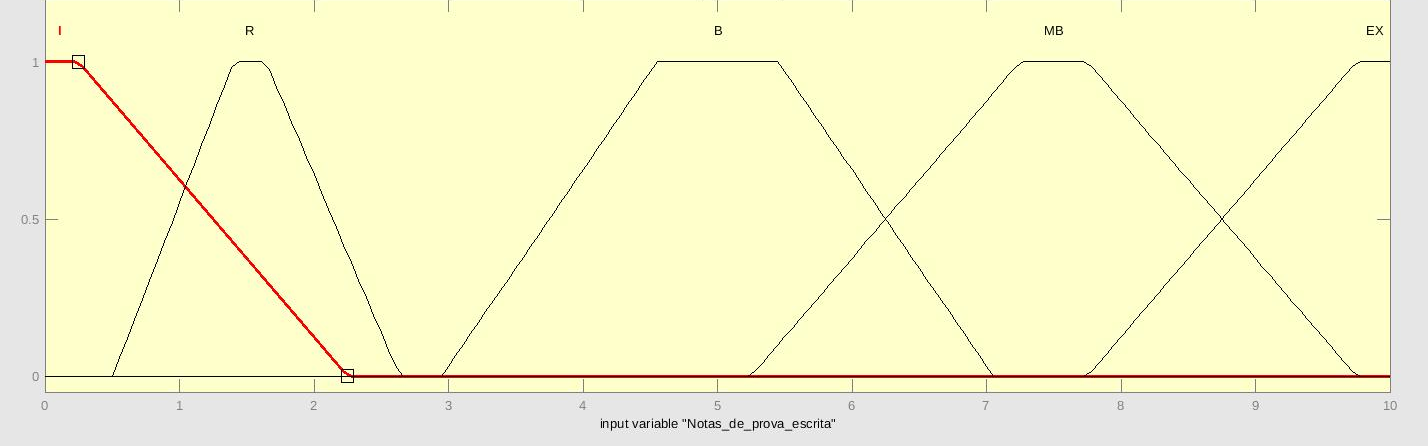
\includegraphics[scale=.2]{X1.png}
\caption{Funções de pertinência para a variável de entrada
``Notas de prova escrita'' (X1)}
\label{fig:notas_de_provas_escritas}
\end{figure}


\begin{figure}[h!]
\centering
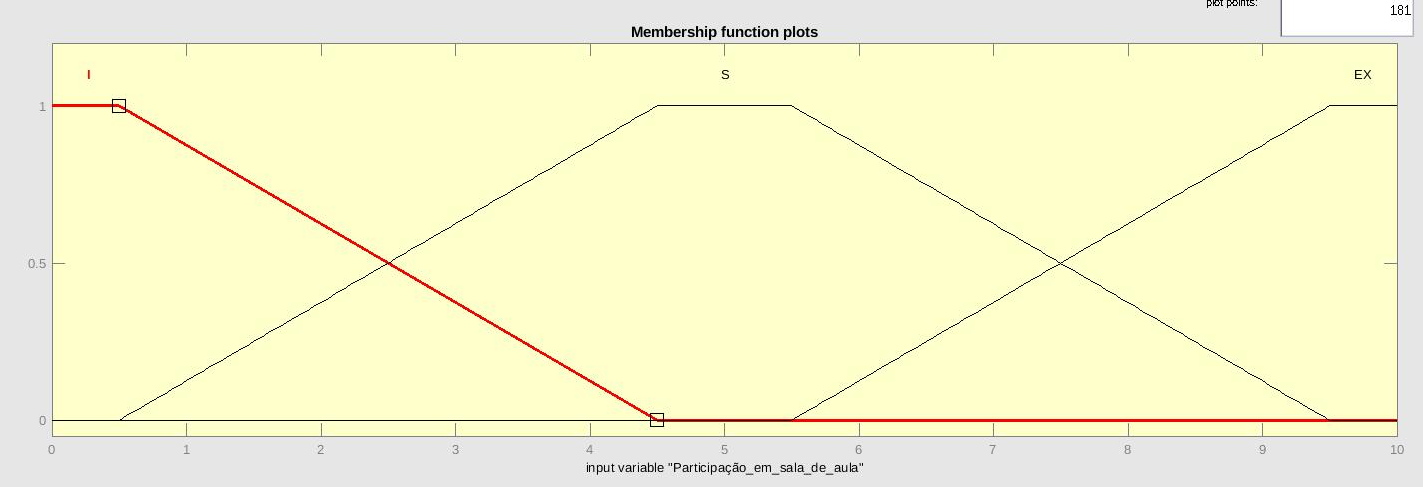
\includegraphics[scale=.2]{X2.png}
\caption{Funções de pertinência para a variável de entrada
``participação em sala de aula'' (X2)}
\label{fig:notas_de_provas_escritas}
\end{figure}

\begin{figure}[h!]
\centering
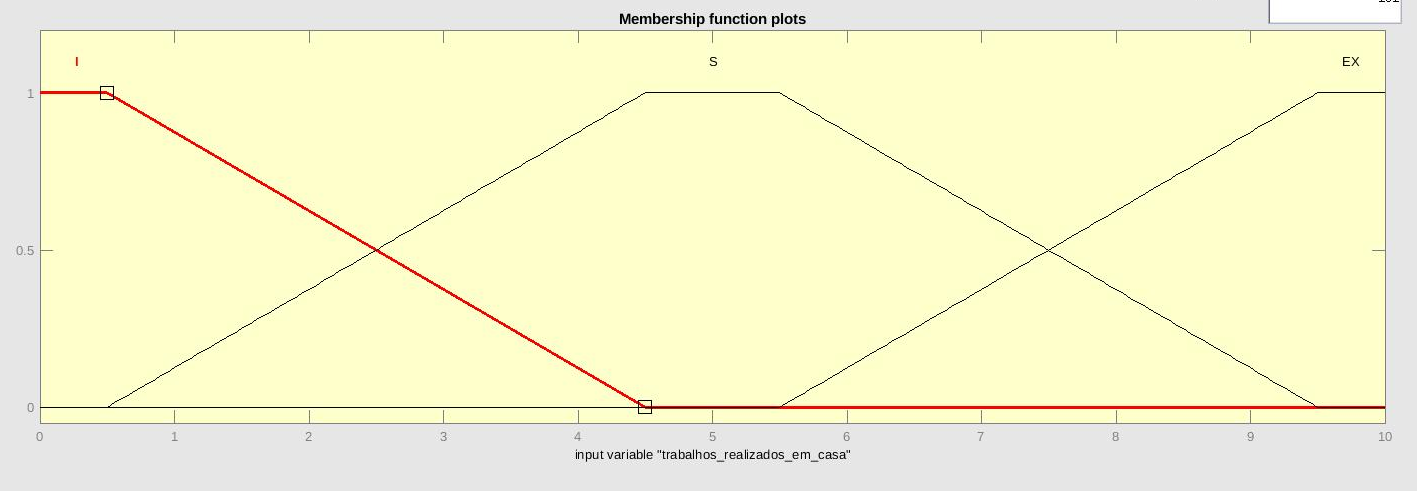
\includegraphics[scale=.2]{X3.png}
\caption{Funções de pertinência para a variável de entrada
``trabalhos realizados em casa'' (X3)}
\label{fig:notas_de_provas_escritas}
\end{figure}

\newpage

\begin{figure}[h!]
\centering
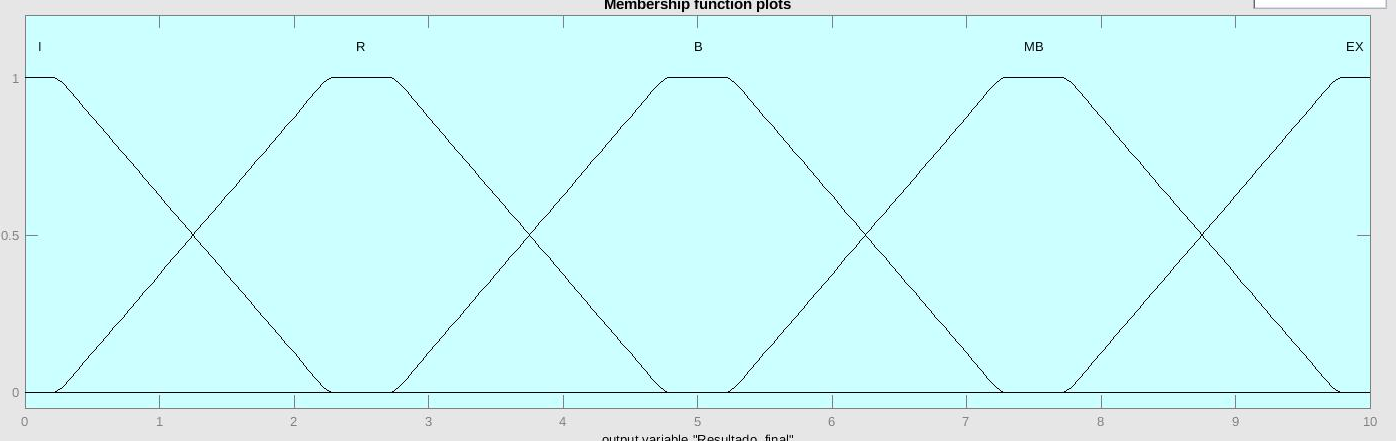
\includegraphics[scale=.2]{Y.png}
\caption{Funções de pertinência para a variável de saída
``resultado final'' (Y)}
\label{fig:notas_de_provas_escritas}
\end{figure}

A base de dados foi escolhida de forma aleatória tentando
contemplar a maior quantidade possível de situações para avaliar
o desempenho dos alunos. O sistema foi composto por 20 regras,
todas modeladas com o mesmo peso e de decisões simples, como por
exemplo: se todas as variáveis de entrada foram consideradas
insuficientes, então o conceito final do estudante deve ser
classificado como insuficiente.

Seguem as 20 regras utilizadas em nosso sistema:

\begin{enumerate}
	\item Se avaliação escrita é insuficiente e atividade em
		classe é insuficiente e atividade extraclasse é
		insuficiente então conceito final é insuficiente.

	\item Se avaliação escrita é insuficiente e atividade em
		classe é insuficiente e atividade extraclasse é não
		insuficiente então conceito final é regular.

	\item Se avaliação escrita é insuficiente e atividade em
		classe é não insuficiente e atividade extraclasse é
		insuficiente então conceito final é regular.

	\item  Se avaliação escrita é insuficiente e atividade em
		classe é não insuficiente e atividade extraclasse é não
		insuficiente então conceito final é regular.

	\item Se avaliação escrita é regular e atividade em classe
		é insuficiente e atividade extraclasse é insuficiente
		então conceito final é insuficiente.

	\item Se avaliação escrita é regular e atividade em classe
		é não insuficiente e atividade extraclasse é
		insuficiente então conceito final é regular.

	\item  Se avaliação escrita é regular e atividade em classe
		é insuficiente e atividade extraclasse é não
		insuficiente então conceito final é bom.

	\item  Se avaliação escrita é regular e atividade em classe
		é não insuficiente e atividade extraclasse é não
		insuficiente então conceito final é bom.

	\item  Se avaliação escrita é bom e atividade em classe é
		insuficiente e atividade extraclasse é insuficiente
		então conceito final é regular.

	\item Se avaliação escrita é bom e atividade em classe é
		insuficiente e atividade extraclasse é não insuficiente
		então conceito final é bom.

	\item Se avaliação escrita é bom e atividade em classe é não
		insuficiente e participação extraclasse é insuficiente
		então conceito final é bom.

	\item Se avaliação escrita é bom e atividade em classe é não
		insuficiente e atividade extraclasse é não insuficiente
		então conceito final é muito bom.

	\item Se avaliação escrita é muito bom e atividade em classe
		é insuficiente e atividade extraclasse é insuficiente
		então conceito final é bom.

	\item Se avaliação escrita é muito bom e atividade em classe
		é não insuficiente e atividade extraclasse é
		insuficiente então conceito final é bom.

	\item Se avaliação escrita é muito bom e atividade em classe
		é insuficiente e atividade extraclasse é não
		insuficiente então conceito final é bom.


	\item Se avaliação escrita é muito bom e atividade em classe
		é não insuficiente e atividade extraclasse é não
		insuficiente então conceito final é muito bom.

	\item Se avaliação escrita é excelente e atividade em classe
		é insuficiente e atividade extraclasse é insuficiente
		então conceito final é muito bom.

	\item Se avaliação escrita é excelente e atividade em classe
		é não insuficiente e atividade extraclasse é não
		insuficiente então conceito final é excelente.

	\item Se avaliação escrita é excelente e atividade em classe
		é não insuficiente e atividade extraclasse é
		insuficiente então conceito final é muito bom.

	\item Se avaliação escrita é excelente e atividade em classe
		é insuficiente e atividade extraclasse é não
		insuficiente então conceito final é muito bom.

\end{enumerate}



\section{Conclusão}
Sabemos que a função da avaliação é auxiliar o processo de
ensino/aprendizagem dos alunos, porém a maneira que está sendo
aplicada não está surtindo os resultados esperados. Para obter
o conceito final do desempenho do aluno, após a realização
de todas as provas de um determinado período, é calculada a
média aritmética com todas as notas obtidas.

A média aritmética usada para o cálculo da nota final
do aluno não analisa todas as notas em conjunto. Um aluno
conseguiu boas notas na primeira e na segunda prova, porém
na terceira prova ele obteve uma nota inferior. Ao calcular
a média esta diminui consideravelmente por causa da nota
baixa da terceira prova. No caso de uma nota mais baixa ao
fazer o cálculo da média o aluno pode ser prejudicado mesmo
tendo notas boas em outras provas. Uma média insatisfatória
transparece que o aluno não aprendeu. Ele pode ter aprendido
muito bem o conteúdo da primeira e segunda prova, porém ele
ficou com uma deficiência no conteúdo da terceira prova. A
média aritmética não mostra essa realidade.


As provas aplicadas e o cálculo matemático utilizado estão
sendo insuficientes para avaliar o aprendizado dos alunos,
portanto um modelo fuzzy foi desenvolvido neste trabalho
utilizando o software Matlab visando a avaliação para cursos
presenciais.


A lógica fuzzy é uma abordagem intuitiva e tolerante com dados
imprecisos. Pode ser construída através de experiência de
especialistas e sobre as estruturas da descrição qualitativa
utilizada na linguagem cotidiana.

Em nosso modelo utilizamos valores aleatórios como entrada
para o sistema fuzzy, tentando contemplar a maior quantidade
possível de situações para avaliar o desempenho dos alunos.
Estes valores utilizados são: nota de avaliação escrita,
atividade em classe e atividade extra classe. O principal
objetivo era usar todos os tipos de avaliações para estimar
um novo índice para o conceito final dos alunos e comparar os
resultados obtidos com o modelo clássico (cálculo matemático
– média aritmética). O sistema fuzzy tem algumas vantagens
quando comparado com o modelo clássico. Possui muitos recursos
para aperfeiçoar a modelagem e adquirir melhores resultados,
por exemplo o formato das funções de pertinência, o modelo de
inferência que pode ser o Mamdani ou o Sugeno além de permitir
trabalhar com variáveis quantitativas e qualitativas. Para
a modelagem desse sistema foi construída uma base de regras
através de variáveis linguísticas que pode ser modificada
até adquirir os resultados esperados. O modelo desenvolvido
possui 20 regras para estimar o índice e sua implementação e
interpretação são fáceis para o usuário.


O mais importante é que este sistema considera a contribuição
de todas as etapas de avaliação do aluno para gerar o índice
para o conceito final. Esta importante contribuição não
ocorreu com os modelos clássicos, porque eles prejudicam o
conceito final do aluno que não foi muito bem em umas das
etapas de avaliação.


Dentre os testes que podem ser feitos no modelo fuzzy como
proposta de trabalhos futuros são:

\begin{itemize}
    \item Dar pesos diferentes para uma determinada regra;
    \item Ao invés de utilizar o método de implicação
Mamdani pode ser usado o modelo de Takagi-Sugeno-Kang;
    \item Além da trapezoidal pode utilizar outras formas de
    funções de pertinência como a triangular, gaussiana,
    sinoidal;
    \item Diminuir as regras para obter melhores resultados.
\end{itemize}

Assim, a metodologia proposta sugere um novo índice de
cálculo que foi capaz de melhorar os resultados do sistema
de classificação clássico na maioria das situações
simuladas e tem uma grande flexibilidade. Estes elementos
ampliam significativamente a sensibilidade do modelo para
a classificação do conceito final do estudante, e faz da
metodologia uma proposta muito adaptável a qualquer nova norma.



\bibliographystyle{plain}
\bibliography{references}

\end{document}

